% Provenance (never printed): cycle 4 SVT, "La planete Terre": the dynamics of
% the Earth's outer shell, plates and their boundaries, continental drift as a
% history of ideas; see sources/outline_sources.md. Pilot chapter, 2026-10-22.
\chapter{La tectonique des plaques~: le puzzle en mouvement}\label{ch:g7:plate-tectonics}

Étale une \omterm{def:g2:drawing-to-map:map}{carte} du monde sur une table et regarde les deux rivages de
l'\omterm{def:g2:water-on-earth:ocean}{océan} Atlantique. Le grand renflement du Brésil semble fait pour se
glisser dans le creux de la \omterm{def:g1:landscapes-around-us:water}{côte} ouest de l'Afrique, comme si quelqu'un
avait coupé en deux un même morceau de terre et écarté les deux moitiés.
Les premiers à imprimer de bonnes \omterm{def:g2:drawing-to-map:map}{cartes} des deux \omterm{def:g1:landscapes-around-us:water}{côtes} l'ont remarqué
aussitôt. Pendant trois siècles, ce fut une simple curiosité. Au
\textsc{xx}\textsuperscript{e}~siècle, c'est devenu le point de départ de
la théorie qui explique aujourd'hui pourquoi le sol tremble au Japon,
pourquoi les Andes sont si hautes, pourquoi l'Islande s'élargit lentement
--- et pourquoi la \omterm{def:g2:drawing-to-map:map}{carte} posée sur la table n'est qu'un instantané d'un
monde en mouvement.

\begin{omfigure}
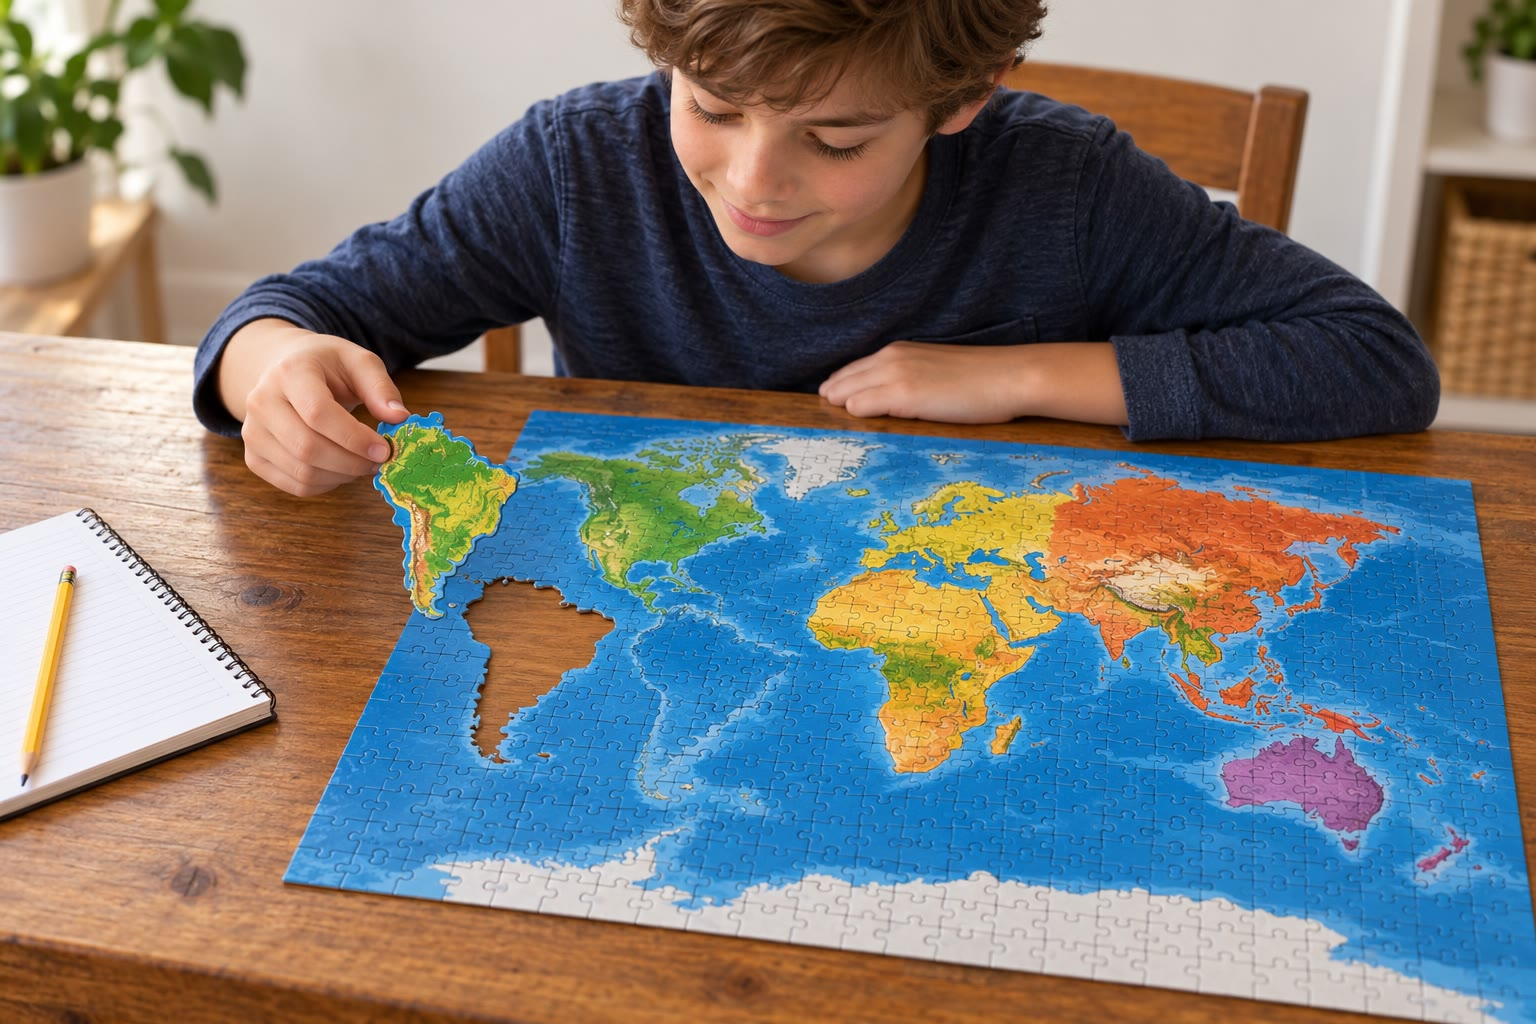
\includegraphics[width=0.62\linewidth]{images/book1/ai/g7-puzzle-map.jpg}

{\small L'Amérique du Sud à côté de l'Afrique~: sur un puzzle,
l'emboîtement est un jeu~; sur la vraie Terre, c'est un indice.}
\end{omfigure}

\begin{recall}
La Terre a trois couches principales~: une fine \emph{\omterm{def:g6:inside-the-earth:layers}{croûte}} rocheuse, un
épais \emph{\omterm{def:g6:inside-the-earth:layers}{manteau}} de \omterm{def:g3:stones-pebbles-sand:rock}{roche} chaude et un \emph{\omterm{def:g6:inside-the-earth:layers}{noyau}} métallique~; la
température augmente avec la profondeur (\cref{ch:g6:inside-the-earth}).
Un lieu du \omterm{def:g3:continents-and-oceans:globe}{globe} est repéré par sa \omterm{def:g6:latitude-longitude:latitude}{latitude} et sa \omterm{def:g6:latitude-longitude:longitude}{longitude}
(\cref{ch:g6:latitude-longitude}).
\end{recall}

\section{Des continents qui s'emboîtaient autrefois}

\begin{definition}[Dérive des continents]\label{def:g7:plate-tectonics:continental-drift}
La \emph{dérive des continents}\index{derive des continents@dérive des continents}
est l'idée que les \omterm{def:g3:continents-and-oceans:continent}{continents} se déplacent lentement à la surface de la
Terre, si bien que leurs positions, et la forme des \omterm{def:g2:water-on-earth:ocean}{océans} qui les
séparent, ont changé au fil des âges.
\end{definition}

\begin{definition}[Supercontinent]\label{def:g7:plate-tectonics:supercontinent}
Un \emph{supercontinent}\index{supercontinent} est une seule masse de terre
formée de tous les \omterm{def:g3:continents-and-oceans:continent}{continents}, ou presque, réunis. Le dernier, la
\emph{Pangée}\index{Pangee@Pangée} («~toutes les terres~» en grec), a
commencé à se fragmenter il y a environ 225 à 200 millions d'années.
% ledger: usgs:pangaea-breakup
\end{definition}

Le scientifique qui a défendu la \omterm{def:g7:plate-tectonics:continental-drift}{dérive des continents} comme une véritable
théorie, preuves à l'appui, est Alfred Wegener. Il a réuni quatre sortes
d'indices.

\begin{enumerate}
  \item \textbf{La forme des \omterm{def:g1:landscapes-around-us:water}{côtes}.} L'Amérique du Sud et l'Afrique
        s'emboîtent comme deux pièces d'un puzzle, et il en va de même pour
        plusieurs autres \omterm{def:g1:landscapes-around-us:water}{côtes}.
  \item \textbf{Les fossiles.} On trouve les mêmes animaux et les mêmes
        plantes fossiles sur des \omterm{def:g3:continents-and-oceans:continent}{continents} aujourd'hui séparés par des
        milliers de kilomètres d'\omterm{def:g2:water-on-earth:ocean}{océan}. \emph{Mesosaurus} était un petit
        reptile qui vivait en \omterm{def:g2:water-on-earth:salt-fresh}{eau douce}~: il n'aurait pas pu traverser un
        \omterm{def:g2:water-on-earth:ocean}{océan} à la nage, et pourtant ses fossiles se trouvent à la fois au
        Brésil et en Afrique australe.
  \item \textbf{Les \omterm{def:g3:stones-pebbles-sand:rock}{roches}.} Des \omterm{def:g3:stones-pebbles-sand:rock}{roches} de mêmes types et de mêmes âges, et
        de vieilles \omterm{def:g4:world-physical-map:range}{chaînes de montagnes} de même forme, s'arrêtent sur une
        \omterm{def:g1:landscapes-around-us:water}{côte} et reprennent sur la \omterm{def:g1:landscapes-around-us:water}{côte} d'en face, comme les lignes d'un
        journal déchiré.
  \item \textbf{Les \omterm{def:g5:weather-and-climate:climate}{climats} anciens.} On trouve en Antarctique du charbon,
        formé à partir des plantes de forêts chaudes et marécageuses~; on
        trouve des traces laissées par d'anciens glaciers dans des régions
        d'Afrique aujourd'hui chaudes et sèches. Ces terres ont dû se
        trouver autrefois sous d'autres \omterm{def:g5:weather-and-climate:climate}{climats}, à d'autres \omterm{def:g6:latitude-longitude:latitude}{latitudes}.
\end{enumerate}
% ledger: usgs:coal-antarctica, usgs:fossil-map

\begin{omfigure}
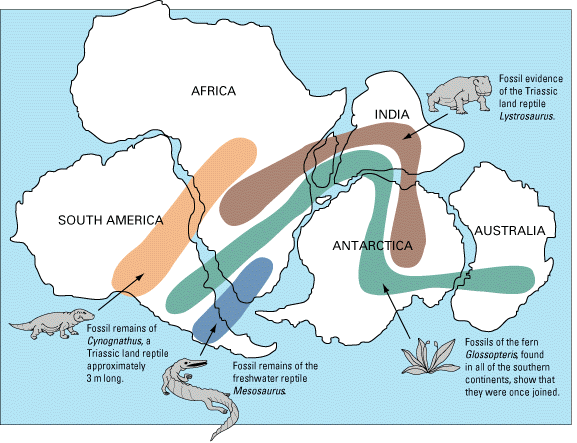
\includegraphics[width=0.86\linewidth]{images/book1/g7-usgs-fossil-map.png}

{\small Les \omterm{def:g3:continents-and-oceans:continent}{continents} du Sud remis ensemble. Chaque bande colorée relie
les lieux où l'on trouve aujourd'hui une espèce fossile~: les reptiles
terrestres \emph{Cynognathus} et \emph{Lystrosaurus}, le reptile d'\omterm{def:g2:water-on-earth:salt-fresh}{eau
douce} \emph{Mesosaurus} et la fougère \emph{Glossopteris}. Séparés, les
\omterm{def:g3:continents-and-oceans:continent}{continents} dispersent les bandes~; réunis, les bandes se poursuivent sans
interruption. \omterm{def:g2:drawing-to-map:map}{Carte}~: U.S. Geological Survey, \emph{This Dynamic Earth}
(domaine public).}
\end{omfigure}

\begin{history}[L'idée de Wegener, 1912--1930]
% ledger: usgs:wegener-1912, usgs:wegener-death, usgs:jeffreys
Alfred Wegener, un météorologue allemand de 32~ans, a exposé la théorie de
la \omterm{def:g7:plate-tectonics:continental-drift}{dérive des continents} dans deux articles en 1912. La plupart des
géologues l'ont rejetée. L'objection la plus forte était que Wegener ne
pouvait pas dire \emph{ce qui} déplaçait les \omterm{def:g3:continents-and-oceans:continent}{continents}~: il pensait qu'ils
labouraient la \omterm{def:g3:stones-pebbles-sand:rock}{roche} du fond des \omterm{def:g2:water-on-earth:ocean}{océans}, et le physicien Harold Jeffreys a
montré que des \omterm{def:g3:continents-and-oceans:continent}{continents} solides ne pouvaient pas faire cela sans se
briser. Wegener a continué de rassembler des preuves jusqu'à sa mort sur
la calotte glaciaire du Groenland, en 1930, au cours d'une expédition. La
réponse qui lui manquait est venue du fond des \omterm{def:g2:water-on-earth:ocean}{océans}, exploré après les
années 1950~: elle sera racontée dans une classe ultérieure.
\end{history}

\section{Les plaques}

Les indices de Wegener étaient justes, mais ses \omterm{def:g3:continents-and-oceans:continent}{continents} n'étaient pas
les bonnes pièces. Ce ne sont pas seulement les \omterm{def:g3:continents-and-oceans:continent}{continents} qui bougent~:
toute l'enveloppe externe de la Terre, sous les \omterm{def:g3:continents-and-oceans:continent}{continents} comme sous les
\omterm{def:g2:water-on-earth:ocean}{océans}, est découpée en morceaux.

\begin{definition}[Plaque tectonique]\label{def:g7:plate-tectonics:plate}
Une \emph{plaque tectonique}\index{plaque tectonique} (ou simplement une
plaque) est un grand bloc de \omterm{def:g3:stones-pebbles-sand:rock}{roche} rigide qui forme une partie de
l'enveloppe externe de la Terre. Une plaque est faite de la \omterm{def:g6:inside-the-earth:layers}{croûte} et de la
partie la plus haute du \omterm{def:g6:inside-the-earth:layers}{manteau}, froide et rigide, l'ensemble ayant au
moins 80 kilomètres d'épaisseur en moyenne~; elle se déplace lentement
sur le \omterm{def:g6:inside-the-earth:layers}{manteau} plus chaud et plus mou situé en dessous.
% ledger: usgs:lithosphere-80km
\end{definition}

\begin{definition}[Tectonique des plaques]\label{def:g7:plate-tectonics:plate-tectonics}
La \emph{tectonique des plaques}\index{tectonique des plaques} est la
théorie selon laquelle l'enveloppe externe de la Terre est divisée en
\omterm{def:g7:plate-tectonics:plate}{plaques} qui se déplacent les unes par rapport aux autres, et selon laquelle
la plupart des \omterm{def:g4:volcanoes-earthquakes-first-look:earthquake}{séismes}, des \omterm{def:g4:volcanoes-earthquakes-first-look:volcano}{volcans} et des \omterm{def:g4:world-physical-map:range}{chaînes de montagnes} se forment
là où des \omterm{def:g7:plate-tectonics:plate}{plaques} se rencontrent.
\end{definition}

\begin{remark}[Combien de plaques~?]\label{rem:g7:plate-tectonics:how-many}
% ledger: usgs:plates-dozen, pb2002:count
Une douzaine de \omterm{def:g7:plate-tectonics:plate}{plaques} environ sont grandes~; beaucoup d'autres sont
petites. Une \omterm{def:g2:drawing-to-map:map}{carte} détaillée utilisée par les géologues en compte 52. Une
\omterm{def:g7:plate-tectonics:plate}{plaque} peut porter un \omterm{def:g3:continents-and-oceans:continent}{continent}, un \omterm{def:g2:water-on-earth:ocean}{océan}, ou les deux~: la \omterm{def:g7:plate-tectonics:plate}{plaque}
sud-américaine porte toute l'Amérique du Sud et la moitié ouest de
l'Atlantique Sud. La \omterm{def:g7:plate-tectonics:plate}{plaque} pacifique, la plus grande, ne porte presque
aucune terre.
\end{remark}

\begin{omfigure}
\begin{tikzpicture}
\begin{axis}[ommap, width=\linewidth, xtick={-180,-90,...,180}, ytick={-60,0,60}]
\addplot[fill=omLithAlluv, draw=black!45, line width=0.2pt] table {figdata/out/shared-geo-land.dat};
\addplot[omRidge, line width=0.8pt] table {figdata/out/shared-geo-school-ridge.dat};
\addplot[omRidge!70!black, line width=0.8pt] table {figdata/out/shared-geo-school-transform.dat};
\addplot[omTrench, line width=0.8pt] table {figdata/out/shared-geo-school-subduction.dat};
\addplot[fill=omTrench, draw=none] table {figdata/out/shared-geo-school-teeth.dat};
\addplot[black!65, line width=0.8pt] table {figdata/out/shared-geo-school-collision.dat};
\begin{scope}[every node/.style={font=\scriptsize\bfseries, text=black!85,
    fill=white, fill opacity=0.75, text opacity=1, inner sep=1pt, align=center}]
  \node at (axis cs:-150,12) {Pacifique};
  \node at (axis cs:-103,52) {Nord-\\américaine};
  \node at (axis cs:-48,-12) {Sud-\\américaine};
  \node at (axis cs:85,57) {Eurasienne};
  \node at (axis cs:18,8) {Africaine};
  \node at (axis cs:10,-75) {Antarctique};
  \node at (axis cs:78,11) {Indienne};
  \node at (axis cs:128,-26) {Australienne};
  \node at (axis cs:-95,-22) {Nazca};
  \node at (axis cs:50,20) {Arabique};
\end{scope}
\end{axis}
\end{tikzpicture}

{\small Les principales \omterm{def:g7:plate-tectonics:plate}{plaques tectoniques}. En rouge~: des \omterm{def:g7:plate-tectonics:plate}{plaques} qui
s'écartent~; en bleu avec des triangles~: une \omterm{def:g7:plate-tectonics:plate}{plaque} qui s'enfonce sous
l'autre (les triangles sont sur la \omterm{def:g7:plate-tectonics:plate}{plaque} qui reste au-dessus)~; en gris~:
des \omterm{def:g7:plate-tectonics:plate}{plaques} qui se poussent l'une contre l'autre sur une large zone de
\omterm{def:g1:landscapes-around-us:landform}{montagnes}~; en rouge foncé~: des \omterm{def:g7:plate-tectonics:plate}{plaques} qui glissent l'une le long de
l'autre. Limites d'après P.~Bird (2003)~; côtes d'après Natural Earth.}
\end{omfigure}

Comment savons-nous où une \omterm{def:g7:plate-tectonics:plate}{plaque} s'arrête et où commence la suivante~?
Regarde où la Terre est agitée.

\begin{proposition}[Les séismes et les volcans dessinent les limites des plaques]\label{prop:g7:plate-tectonics:restless}
% ledger: data:usgs-comcat, data:pb2002 (share computed in figdata/grade-7/quakes_on_boundaries.py)
Les \omterm{def:g4:volcanoes-earthquakes-first-look:earthquake}{séismes} et les \omterm{def:g4:volcanoes-earthquakes-first-look:volcano}{volcans} ne sont pas dispersés au hasard sur la Terre~:
la plupart se trouvent le long d'étroites bandes, et ces bandes sont les
bords des \omterm{def:g7:plate-tectonics:plate}{plaques}. Sur les 7\,031 \omterm{def:g4:volcanoes-earthquakes-first-look:earthquake}{séismes} de magnitude 6 ou plus
enregistrés entre 1976 et 2025, 6\,472 --- soit 92\,\% --- se sont
produits à moins de \qty{300}{km} d'une \omterm{def:g7:plate-tectonics:plate-boundary}{limite de plaques}.
\end{proposition}

\begin{omfigure}
\begin{tikzpicture}
\begin{axis}[ommap, width=\linewidth, xtick={-180,-90,...,180}, ytick={-60,0,60},
  legend style={at={(0.02,0.04)}, anchor=south west, font=\scriptsize,
  fill=white, fill opacity=0.85, text opacity=1, draw=black!40}]
\addplot[fill=omLithAlluv, draw=black!45, line width=0.2pt, forget plot] table {figdata/out/shared-geo-land.dat};
\addplot[only marks, mark=*, mark size=0.45pt, omThm!85!black] table[x=lon, y=lat] {figdata/out/grade-7-quakes_on_boundaries-map.dat};
\addlegendentry{séisme de magnitude 6.5 ou plus, 1976--2025}
\addplot[only marks, mark=triangle*, mark size=1.1pt, black] table {figdata/out/shared-geo-volcanoes.dat};
\addlegendentry{volcan actif au cours des 12\,000 dernières années}
\end{axis}
\end{tikzpicture}

{\small Les grands \omterm{def:g4:volcanoes-earthquakes-first-look:earthquake}{séismes} et les \omterm{def:g4:volcanoes-earthquakes-first-look:volcano}{volcans} récents. Compare avec la \omterm{def:g2:drawing-to-map:map}{carte} des
\omterm{def:g7:plate-tectonics:plate}{plaques} ci-dessus~: les points et les triangles dessinent les \omterm{def:g7:plate-tectonics:plate-boundary}{limites des
plaques}. Données~: catalogue des \omterm{def:g4:volcanoes-earthquakes-first-look:earthquake}{séismes} de l'U.S. Geological Survey~;
Global Volcanism Program de la Smithsonian Institution.}
\end{omfigure}

\section{Trois sortes de limites de plaques}

\begin{definition}[Limite de plaques]\label{def:g7:plate-tectonics:plate-boundary}
Une \emph{limite de plaques}\index{limite de plaques} est la ligne, ou la
zone étroite, où deux \omterm{def:g7:plate-tectonics:plate}{plaques} se rencontrent. Selon la façon dont les deux
\omterm{def:g7:plate-tectonics:plate}{plaques} se déplacent l'une par rapport à l'autre, une limite est de l'une
de ces trois sortes~:
\begin{itemize}
  \item à une \emph{limite divergente}\index{limite divergente}, les deux
        \omterm{def:g7:plate-tectonics:plate}{plaques} s'écartent~;
  \item à une \emph{limite convergente}\index{limite convergente}, les deux
        \omterm{def:g7:plate-tectonics:plate}{plaques} se rapprochent~;
  \item à une \emph{limite transformante}\index{limite transformante}, les
        deux \omterm{def:g7:plate-tectonics:plate}{plaques} glissent l'une le long de l'autre, \omterm{def:g1:landscapes-around-us:water}{côte} à \omterm{def:g1:landscapes-around-us:water}{côte}.
\end{itemize}
\end{definition}

\begin{example}[Limites divergentes~: l'Islande et l'Afrique de l'Est]\label{ex:g7:plate-tectonics:divergent}
% ledger: usgs:iceland, usgs:east-africa
Au milieu de l'\omterm{def:g2:water-on-earth:ocean}{océan} Atlantique court une \omterm{def:g4:world-physical-map:range}{chaîne de montagnes} sous-marines,
la dorsale médio-atlantique, où les \omterm{def:g7:plate-tectonics:plate}{plaques} situées de part et d'autre
s'écartent. De la \omterm{def:g3:stones-pebbles-sand:rock}{roche} chaude du \omterm{def:g6:inside-the-earth:layers}{manteau} monte dans l'intervalle, fond en
partie et devient un nouveau fond océanique~: une \omterm{def:g7:plate-tectonics:plate-boundary}{limite divergente}
construit de la \omterm{def:g7:plate-tectonics:plate}{plaque} nouvelle. L'Islande est un morceau de cette dorsale
qui émerge au-dessus de la \omterm{def:g2:water-on-earth:ocean}{mer}~: là, l'Amérique du Nord se déplace vers
l'ouest et l'Eurasie vers l'est, et l'île se déchire lentement. Entre 1975
et 1984, les fissures proches du \omterm{def:g4:volcanoes-earthquakes-first-look:volcano}{volcan} Krafla, dans le nord de l'île, se
sont élargies d'environ 7 mètres au total. Une \omterm{def:g7:plate-tectonics:plate-boundary}{limite divergente} peut aussi
traverser un \omterm{def:g3:continents-and-oceans:continent}{continent}~: le long du rift est-africain, l'Afrique commence à
se fendre, et la \omterm{def:g2:water-on-earth:ocean}{mer} Rouge est un jeune \omterm{def:g2:water-on-earth:ocean}{océan} qui a déjà séparé l'Arabie de
l'Afrique.
\end{example}

\begin{example}[Limites convergentes~: les Andes et l'Himalaya]\label{ex:g7:plate-tectonics:convergent}
% ledger: usgs:trench-depth, usgs:himalaya
Au large de la \omterm{def:g1:landscapes-around-us:water}{côte} ouest de l'Amérique du Sud, la \omterm{def:g7:plate-tectonics:plate}{plaque} de Nazca, qui
porte un \omterm{def:g2:water-on-earth:ocean}{océan}, se rapproche de la \omterm{def:g7:plate-tectonics:plate}{plaque} sud-américaine, qui porte un
\omterm{def:g3:continents-and-oceans:continent}{continent}. La \omterm{def:g7:plate-tectonics:plate}{plaque} océanique, plus lourde, se courbe et s'enfonce sous le
\omterm{def:g3:continents-and-oceans:continent}{continent}, loin dans le \omterm{def:g6:inside-the-earth:layers}{manteau}. Le long de la ligne où elle plonge, le
fond de la \omterm{def:g2:water-on-earth:ocean}{mer} descend dans une fosse profonde~; au-dessus de la \omterm{def:g7:plate-tectonics:plate}{plaque} qui
s'enfonce, la terre est secouée par des \omterm{def:g4:volcanoes-earthquakes-first-look:earthquake}{séismes} et bordée de \omterm{def:g4:volcanoes-earthquakes-first-look:volcano}{volcans}~: ce
sont les Andes. Dans l'ouest du Pacifique, là où une \omterm{def:g7:plate-tectonics:plate}{plaque} océanique
s'enfonce sous une autre, les fosses sont les endroits les plus profonds
de la Terre~: la fosse des Mariannes atteint près de \qty{11000}{m} de
profondeur. Quand deux \omterm{def:g3:continents-and-oceans:continent}{continents} se rencontrent, aucun ne s'enfonce~: la
\omterm{def:g6:inside-the-earth:layers}{croûte} se plisse et s'épaissit. L'Inde est entrée en collision avec l'Asie
il y a environ 50 millions d'années, et les deux \omterm{def:g7:plate-tectonics:plate}{plaques} continuent de se
pousser~; c'est ainsi que se sont élevés l'Himalaya et le plateau tibétain.
\end{example}

\begin{example}[Une limite transformante~: la faille de San Andreas]\label{ex:g7:plate-tectonics:transform}
% ledger: usgs:san-andreas, usgs:san-andreas-photo
En Californie, la \omterm{def:g7:plate-tectonics:plate}{plaque} pacifique glisse vers le nord-ouest le long de la
\omterm{def:g7:plate-tectonics:plate}{plaque} nord-américaine, sur la faille de San Andreas, longue d'environ
\qty{1300}{km}. Aucune \omterm{def:g7:plate-tectonics:plate}{plaque} n'y est créée ni détruite~; les deux \omterm{def:g7:plate-tectonics:plate}{plaques}
frottent l'une contre l'autre, et les secousses de ce frottement sont des
\omterm{def:g4:volcanoes-earthquakes-first-look:earthquake}{séismes}.
\end{example}

\begin{omfigure}
\begin{tikzpicture}[x=1cm, y=1cm, font=\small]
  % mantle
  \fill[omLithGranite!45] (0,-3.3) rectangle (12.4,-0.85);
  \node[font=\footnotesize, text=black!75] at (2.6,-2.6) {manteau~: chaud et mou};
  % sea water
  \fill[omSea] (0,0) -- (0,-0.75) -- (1.5,-0.6) -- (3,-0.25) -- (4.5,-0.6)
    -- (7.4,-0.8) -- (8.0,-1.2) -- (8.6,-0.6) -- (8.9,0) -- cycle;
  % oceanic plates (the ridge at x = 3, the trench at x = 8)
  \fill[omLithBasalt!70] (0,-0.75) -- (1.5,-0.6) -- (3,-0.25) -- (4.5,-0.6)
    -- (7.4,-0.8) -- (8.0,-1.2) -- (9.6,-2.3) -- (10.2,-3.3) -- (9.5,-3.3)
    -- (8.6,-2.2) -- (7.5,-1.55) -- (4.5,-1.35) -- (3.2,-0.95) -- (2.8,-0.95)
    -- (1.5,-1.35) -- (0,-1.45) -- cycle;
  % continental plate
  \fill[omLithSand!80] (8.6,-0.6) -- (8.9,0) -- (9.4,0.35) -- (9.8,0.9)
    -- (10.2,0.35) -- (12.4,0.2) -- (12.4,-1.9) -- (10.6,-1.9) -- (9.6,-2.3)
    -- (8.0,-1.2) -- cycle;
  \draw[black!70, line width=0.5pt] (0,-0.75) -- (1.5,-0.6) -- (3,-0.25)
    -- (4.5,-0.6) -- (7.4,-0.8) -- (8.0,-1.2) -- (8.6,-0.6) -- (8.9,0)
    -- (9.4,0.35) -- (9.8,0.9) -- (10.2,0.35) -- (12.4,0.2);
  \draw[black!45, densely dashed] (0,0) -- (8.9,0);
  % magma: under the ridge and under the volcano
  \fill[omThm!80] (2.85,-0.95) -- (3,-0.3) -- (3.15,-0.95) -- cycle;
  \draw[omThm!80, line width=1.4pt, -{Stealth[length=2.2mm]}] (3,-1.85) -- (3,-1.0);
  \draw[omThm!80, line width=1.2pt, decorate, decoration={snake, amplitude=0.6pt,
    segment length=4pt}] (9.8,-2.45) -- (9.8,0.75);
  % plate motions
  \draw[black, line width=1pt, -{Stealth[length=2.4mm]}] (2.5,-0.75) -- (1.3,-0.95);
  \draw[black, line width=1pt, -{Stealth[length=2.4mm]}] (3.5,-0.75) -- (5.4,-1.05);
  \draw[black, line width=1pt, -{Stealth[length=2.4mm]}] (12.1,-0.85) -- (10.9,-0.85);
  \draw[black, line width=1pt, -{Stealth[length=2.4mm]}] (8.7,-1.75) -- (9.3,-2.25);
  % labels
  \node[font=\footnotesize, align=center, above] at (3,0.05) {limite divergente~:\\dorsale océanique};
  \node[font=\footnotesize, align=center, below] at (6.9,-1.95) {limite convergente~:\\la plaque océanique s'enfonce};
  \draw[black!60, thin] (8.0,-1.25) -- (7.6,-1.9);
  \node[font=\footnotesize, above] at (8.0,0.05) {fosse};
  \draw[black!60, thin] (8.0,0.05) -- (8.0,-1.1);
  \node[font=\footnotesize, above] at (9.8,0.95) {volcan};
  \node[font=\footnotesize] at (11.4,-0.4) {continent};
  \node[font=\footnotesize] at (1.2,-1.6) {plaque océanique};
  \node[font=\footnotesize, text=black!70] at (5.6,-0.32) {océan};
\end{tikzpicture}

\medskip
\begin{tikzpicture}[font=\small]
  \fill[omLithBasalt!45] (0,0) rectangle (2.4,2.2);
  \fill[omLithSand!70] (2.4,0) rectangle (4.8,2.2);
  \draw[fault] (2.4,-0.1) -- (2.4,2.3);
  \draw[black, line width=1pt, -{Stealth[length=2.4mm]}] (1.2,0.5) -- (1.2,1.7);
  \draw[black, line width=1pt, -{Stealth[length=2.4mm]}] (3.6,1.7) -- (3.6,0.5);
  \node[font=\footnotesize, below] at (1.2,-0.1) {plaque A};
  \node[font=\footnotesize, below] at (3.6,-0.1) {plaque B};
  \node[font=\footnotesize, align=left, anchor=west] at (5.1,1.1)
    {limite transformante, vue de dessus~:\\les plaques glissent l'une le long de l'autre~;\\aucune plaque n'est créée ni détruite};
\end{tikzpicture}

{\small En haut~: une coupe à travers deux \omterm{def:g7:plate-tectonics:plate-boundary}{limites de plaques} (pas à
l'échelle~; les profondeurs sont très exagérées). À la dorsale, les \omterm{def:g7:plate-tectonics:plate}{plaques}
s'écartent et de la \omterm{def:g3:stones-pebbles-sand:rock}{roche} chaude monte du \omterm{def:g6:inside-the-earth:layers}{manteau}~; à la fosse, la \omterm{def:g7:plate-tectonics:plate}{plaque}
océanique s'enfonce sous le \omterm{def:g3:continents-and-oceans:continent}{continent}, et la \omterm{def:g3:stones-pebbles-sand:rock}{roche} qui fond au-dessus
d'elle alimente des \omterm{def:g4:volcanoes-earthquakes-first-look:volcano}{volcans}. En bas~: une \omterm{def:g7:plate-tectonics:plate-boundary}{limite transformante} vue de
dessus.}
\end{omfigure}

\begin{omfigure}
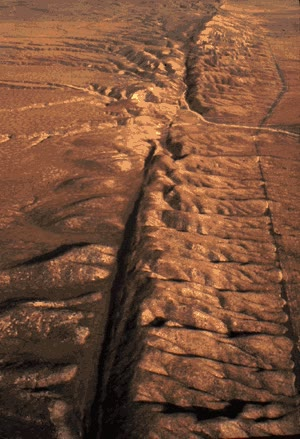
\includegraphics[width=0.28\linewidth]{images/book1/g7-usgs-san-andreas.jpg}

{\small La faille de San Andreas traversant la Carrizo Plain, en Californie,
vue d'avion~: la longue \omterm{def:g1:landscapes-around-us:landform}{vallée} rectiligne est la limite entre la \omterm{def:g7:plate-tectonics:plate}{plaque}
pacifique (à gauche) et la \omterm{def:g7:plate-tectonics:plate}{plaque} nord-américaine (à droite).
Photographie~: Robert E. Wallace, U.S. Geological Survey (domaine public).}
\end{omfigure}

\begin{method}[Reconnaître une limite de plaques sur une carte]\label{met:g7:plate-tectonics:recognise}
Pour savoir quelle sorte de limite sépare deux \omterm{def:g7:plate-tectonics:plate}{plaques}~:
\begin{enumerate}
  \item cherche, sur une \omterm{def:g2:drawing-to-map:map}{carte} des mouvements des \omterm{def:g7:plate-tectonics:plate}{plaques}, les flèches
        situées de part et d'autre de la limite~;
  \item si elles s'éloignent de la limite, elle est divergente~; si elles
        pointent vers elle, convergente~; si elles lui sont \omterm{def:g6:latitude-longitude:latitude}{parallèles} et
        pointent dans des sens opposés, transformante~;
  \item vérifie avec le \omterm{def:g1:landscapes-around-us:landscape}{paysage}~: une dorsale au milieu d'un \omterm{def:g2:water-on-earth:ocean}{océan} ou un
        rift à travers un \omterm{def:g3:continents-and-oceans:continent}{continent} vont avec une \omterm{def:g7:plate-tectonics:plate-boundary}{limite divergente}~; une
        fosse profonde avec une ligne de \omterm{def:g4:volcanoes-earthquakes-first-look:volcano}{volcans}, ou une haute \omterm{def:g4:world-physical-map:range}{chaîne de
        montagnes}, avec une \omterm{def:g7:plate-tectonics:plate-boundary}{limite convergente}~; une longue faille
        rectiligne sans l'un ni l'autre, avec une \omterm{def:g7:plate-tectonics:plate-boundary}{limite transformante}.
\end{enumerate}
\end{method}

\section{À quelle vitesse les plaques se déplacent-elles~?}

\begin{proposition}[Quelques centimètres par an]\label{prop:g7:plate-tectonics:speed}
% ledger: data:pb2002 (speeds computed in figdata/grade-7/plate_speeds.py), usgs:mar-rate
Deux \omterm{def:g7:plate-tectonics:plate}{plaques} voisines se déplacent l'une par rapport à l'autre à une
vitesse de quelques centimètres par an~: d'environ 2 centimètres par an à
travers l'Atlantique Nord à plus de 14 centimètres par an à travers la
dorsale du Pacifique Est, la dorsale la plus rapide de la Terre.
\end{proposition}

\begin{omfigure}
\begin{tikzpicture}
\begin{axis}[xbar, width=0.77\linewidth, height=5.4cm, xmin=0, xmax=16.5,
  ytick={1,...,6}, yticklabels={dorsale de l'Atlantique Nord, dorsale de l'Atlantique Sud,
  faille de San Andreas, Himalaya, fosse du Pérou--Chili, dorsale du Pacifique Est},
  y tick label style={font=\small}, tick label style={font=\small},
  xlabel={vitesse d'une plaque par rapport à l'autre (cm par an)},
  label style={font=\small}, bar width=7pt, axis x line=bottom,
  axis y line=left, axis line style={-}, enlarge y limits=0.12,
  nodes near coords, nodes near coords style={font=\scriptsize},
  every node near coord/.append style={/pgf/number format/fixed,
  /pgf/number format/precision=1, /pgf/number format/fixed zerofill}]
\addplot[fill=omDef!55, draw=omDef!80!black] table[x=speed_cm_a, y=rank] {figdata/out/grade-7-plate_speeds.dat};
\end{axis}
\end{tikzpicture}

{\small La vitesse des \omterm{def:g7:plate-tectonics:plate}{plaques} à six limites~: moyennes le long de chaque
limite, calculées à partir du modèle de \omterm{def:g7:plate-tectonics:plate}{plaques} de P.~Bird (2003).}
\end{omfigure}

\begin{method}[Des centimètres par an aux kilomètres par million d'années]\label{met:g7:plate-tectonics:convert}
Un kilomètre vaut \num{100000} centimètres. Une vitesse de \qty{1}{cm} par
an, maintenue pendant un million d'années, fait donc parcourir
\num{1000000} centimètres, soit \qty{10}{km}. D'où~:
\[
  1\ \text{cm par an} = 10\ \text{km par million d'années}.
\]
Multiplie une vitesse en centimètres par an par 10 pour obtenir des
kilomètres par million d'années~; multiplie ensuite par un nombre de
millions d'années pour obtenir une distance en kilomètres, ou divise une
distance par la vitesse pour obtenir une durée.
\end{method}

\begin{example}[L'Atlantique s'agrandit]\label{ex:g7:plate-tectonics:atlantic}
% ledger: usgs:mar-rate
En moyenne, les deux côtés de la dorsale médio-atlantique s'écartent
d'environ \qty{2.5}{cm} par an, soit \qty{25}{km} par million d'années. En
100 millions d'années, cela fait \qty{2500}{km}~: maintenue assez
longtemps, une vitesse bien trop lente pour être remarquée au cours d'une
vie ouvre un \omterm{def:g2:water-on-earth:ocean}{océan}.
\end{example}

\begin{remark}[Mesurer le mouvement aujourd'hui]\label{rem:g7:plate-tectonics:gps}
% ledger: usgs:gps
Ces mouvements lents se mesurent aujourd'hui directement. Des stations
permanentes fixées sur la \omterm{def:g3:stones-pebbles-sand:rock}{roche en place} reçoivent les signaux de
satellites de positionnement et calculent leur propre position, jour après
jour, à quelques millimètres près. En quelques années, on voit des stations
situées sur des \omterm{def:g7:plate-tectonics:plate}{plaques} différentes s'éloigner ou se rapprocher, aux
vitesses trouvées grâce aux \omterm{def:g3:stones-pebbles-sand:rock}{roches} sur des millions d'années. Le
positionnement par satellite est lui-même le sujet du
\cref{ch:g9:maps-of-the-earth}.
\end{remark}

\begin{omfigure}
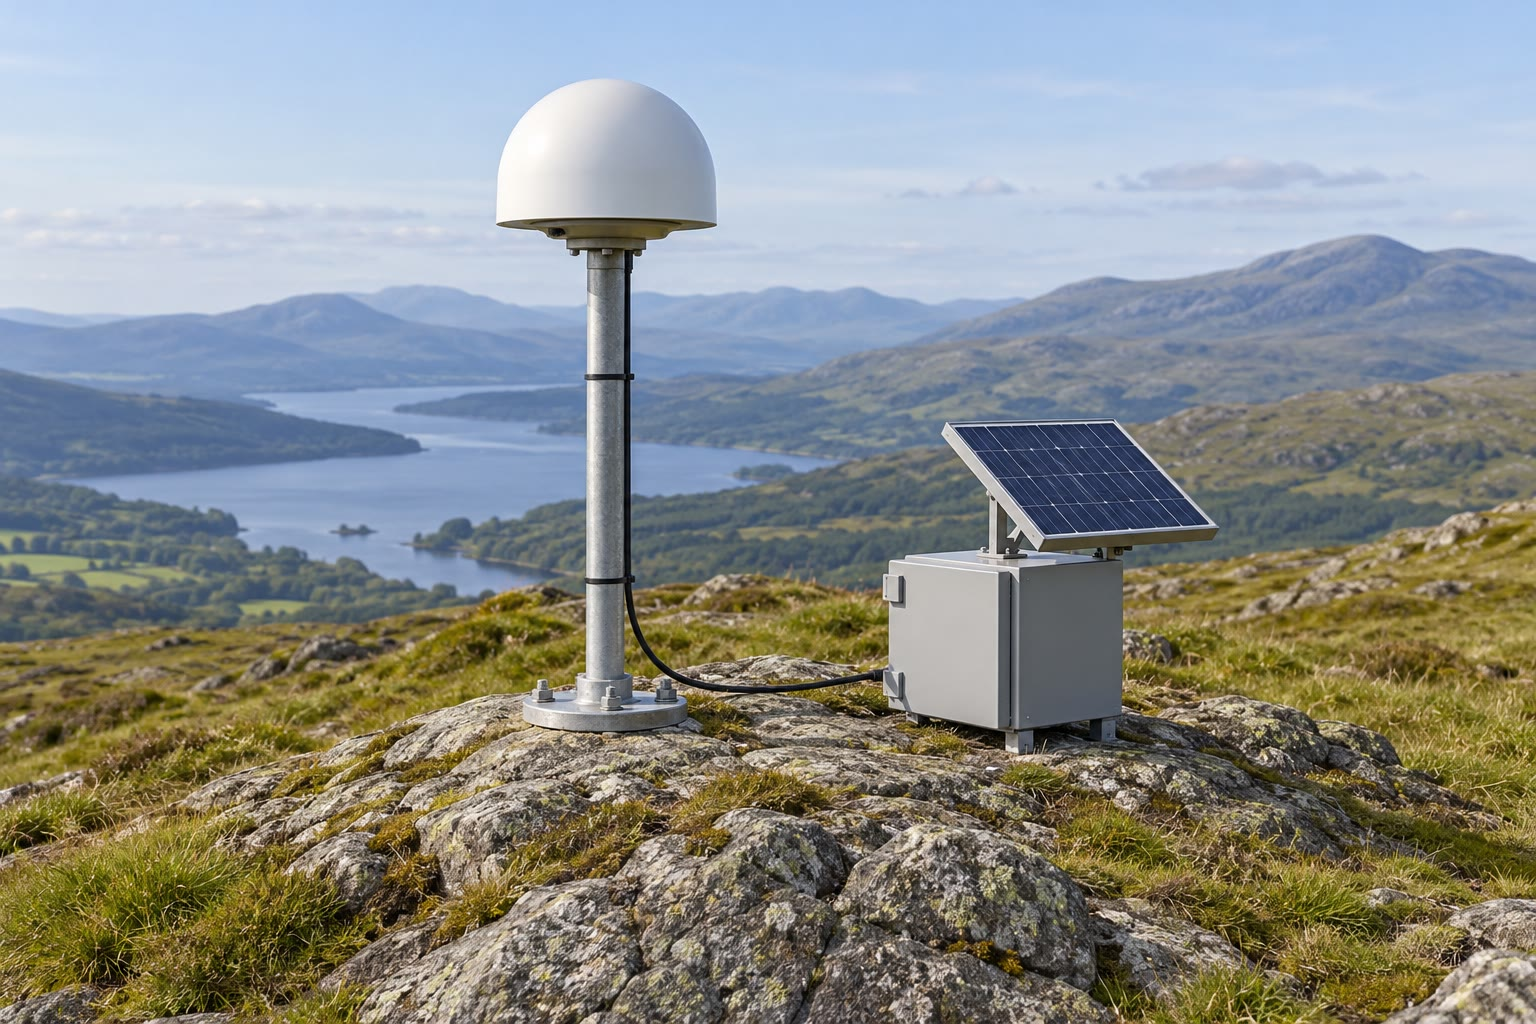
\includegraphics[width=0.55\linewidth]{images/book1/ai/g7-gps-station.jpg}

{\small Une station de positionnement permanente~: son antenne est boulonnée
à la \omterm{def:g3:stones-pebbles-sand:rock}{roche}, si bien qu'elle se déplace avec la \omterm{def:g7:plate-tectonics:plate}{plaque}.}
\end{omfigure}

\section{Exercices}

\begin{exercise}[$\star$]\label{exo:g7:plate-tectonics:1}
Qu'est-ce que la \omterm{def:g7:plate-tectonics:continental-drift}{dérive des continents}~? Donne les quatre sortes d'indices
que Wegener a utilisées pour la défendre.
\end{exercise}

\begin{exercise}[$\star$]\label{exo:g7:plate-tectonics:2}
Nomme les trois sortes de \omterm{def:g7:plate-tectonics:plate-boundary}{limites de plaques} et dis, pour chacune, comment
les deux \omterm{def:g7:plate-tectonics:plate}{plaques} se déplacent l'une par rapport à l'autre.
\end{exercise}

\begin{exercise}[$\star$]\label{exo:g7:plate-tectonics:3}
Regarde la \omterm{def:g2:drawing-to-map:map}{carte} des \omterm{def:g4:volcanoes-earthquakes-first-look:earthquake}{séismes} et des \omterm{def:g4:volcanoes-earthquakes-first-look:volcano}{volcans}. Nomme deux régions du monde
qui ont beaucoup de grands \omterm{def:g4:volcanoes-earthquakes-first-look:earthquake}{séismes}, et un \omterm{def:g3:continents-and-oceans:continent}{continent} qui n'en a presque pas
en son milieu.
\end{exercise}

\begin{exercise}[$\star$]\label{exo:g7:plate-tectonics:4}
On trouve au Brésil et en Afrique australe des fossiles de
\emph{Mesosaurus}, un petit reptile qui vivait en \omterm{def:g2:water-on-earth:salt-fresh}{eau douce}. Pourquoi est-ce
un indice que les deux \omterm{def:g3:continents-and-oceans:continent}{continents} ont été réunis autrefois~?
\end{exercise}

\begin{exercise}[$\star\star$]\label{exo:g7:plate-tectonics:5}
On trouve du charbon en Antarctique. Qu'est-ce que cela nous apprend sur le
\omterm{def:g5:weather-and-climate:climate}{climat} dans lequel ce charbon s'est formé, et que peut-on en conclure sur
l'endroit où se trouvait l'Antarctique à cette époque~?
\end{exercise}

\begin{exercise}[$\star\star$]\label{exo:g7:plate-tectonics:6}
Dis quelle sorte de limite se trouve à chacun de ces endroits~: la dorsale
médio-atlantique~; les Andes~; la faille de San Andreas~; l'Himalaya~; le
rift est-africain.
\end{exercise}

\begin{exercise}[$\star\star$]\label{exo:g7:plate-tectonics:7}
Convertis une vitesse de \qty{2.5}{cm} par an en kilomètres par million
d'années. De combien deux points situés de part et d'autre de la limite
s'éloigneraient-ils en 60 millions d'années à cette vitesse~?
\end{exercise}

\begin{exercise}[$\star\star$]\label{exo:g7:plate-tectonics:8}
Entre 1975 et 1984 --- neuf ans --- les fissures proches du \omterm{def:g4:volcanoes-earthquakes-first-look:volcano}{volcan} Krafla,
en Islande, se sont élargies d'environ \qty{7}{m} au total. Quel a été
l'élargissement moyen par an, en centimètres~? Compare-le avec la vitesse
moyenne de la dorsale médio-atlantique, environ \qty{2.5}{cm} par an, et
propose une raison pour laquelle les deux nombres sont si différents.
\end{exercise}

\begin{exercise}[$\star\star$]\label{exo:g7:plate-tectonics:9}
La théorie de Wegener a été rejetée pendant des dizaines d'années. À quelle
question ne pouvait-il pas répondre~? Qu'est-ce que la théorie de la
\omterm{def:g7:plate-tectonics:plate-tectonics}{tectonique des plaques} change à son image des \omterm{def:g3:continents-and-oceans:continent}{continents} en mouvement~?
\end{exercise}

\begin{exercise}[$\star\star$]\label{exo:g7:plate-tectonics:10}
Regarde la coupe à travers deux \omterm{def:g7:plate-tectonics:plate-boundary}{limites de plaques}. Où le fond de la \omterm{def:g2:water-on-earth:ocean}{mer}
est-il le plus haut, et où est-il le plus profond~? Où de la \omterm{def:g7:plate-tectonics:plate}{plaque}
nouvelle se forme-t-elle, et où une \omterm{def:g7:plate-tectonics:plate}{plaque} retourne-t-elle dans le
\omterm{def:g6:inside-the-earth:layers}{manteau}~?
\end{exercise}

\begin{exercise}[$\star\star\star$]\label{exo:g7:plate-tectonics:11}
À travers la dorsale du Pacifique Est, les \omterm{def:g7:plate-tectonics:plate}{plaques} s'écartent d'environ
\qty{14.2}{cm} par an, et à travers la dorsale de l'Atlantique Nord
d'environ \qty{2.2}{cm} par an. Combien de fois la dorsale du Pacifique Est
est-elle plus rapide (arrondis à l'unité)~? Combien de temps chaque
dorsale met-elle pour ouvrir \qty{1000}{km} de nouveau fond océanique~?
\end{exercise}

\begin{exercise}[$\star\star\star$]\label{exo:g7:plate-tectonics:12}
% ledger: data:usgs-comcat, data:pb2002 (counts in figdata/grade-7/quakes_on_boundaries.py, part bands)
Sur les 7\,031 \omterm{def:g4:volcanoes-earthquakes-first-look:earthquake}{séismes} de magnitude 6 ou plus enregistrés de 1976 à 2025,
4\,578 se sont produits à moins de \qty{100}{km} de la ligne d'une \omterm{def:g7:plate-tectonics:plate-boundary}{limite
de plaques} tracée sur la \omterm{def:g2:drawing-to-map:map}{carte}, 6\,472 à moins de \qty{300}{km} et 6\,786
à moins de \qty{500}{km}.
(a) Combien se sont produits entre \qty{100}{km} et \qty{300}{km} de la
ligne~? (b) Calcule, à l'unité près, le pourcentage de tous ces \omterm{def:g4:volcanoes-earthquakes-first-look:earthquake}{séismes} qui
se sont produits à moins de \qty{100}{km} de la ligne. (c) Beaucoup des
\omterm{def:g4:volcanoes-earthquakes-first-look:earthquake}{séismes} situés entre \qty{100}{km} et \qty{300}{km} de la ligne se
trouvent du même côté d'une fosse océanique profonde. À l'aide de ce qui
se passe à une \omterm{def:g7:plate-tectonics:plate-boundary}{limite convergente}, explique pourquoi un \omterm{def:g4:volcanoes-earthquakes-first-look:earthquake}{séisme} causé par
une \omterm{def:g7:plate-tectonics:plate-boundary}{limite de plaques} peut se produire si loin de la ligne tracée sur la
\omterm{def:g2:drawing-to-map:map}{carte}.
\end{exercise}

\section{Problème~: L'ouverture de l'Atlantique Sud}

\begin{problem}[{Problème du week-end --- mesurer un océan sur la carte et
trouver combien de temps il a mis à s'ouvrir}]
\label{pb:g7:plate-tectonics:1}
% ledger: data:ne-land, earth:Rmean, data:pb2002, usgs:pangaea-breakup, usgs:atlantic-growth
% (all numbers computed in figdata/grade-7/south_atlantic.py: coasts at 23 S
% at 43.21 W and 14.39 E, 102.4 km per degree, AF-SA full rate 3.43 cm/yr)
Sur une \omterm{def:g2:drawing-to-map:map}{carte} de l'Atlantique Sud, une élève suit le \omterm{def:g6:latitude-longitude:latitude}{parallèle} de \omterm{def:g6:latitude-longitude:latitude}{latitude}
\ang{23} Sud. Il quitte la \omterm{def:g1:landscapes-around-us:water}{côte} de l'Amérique du Sud près de Rio de
Janeiro, à la \omterm{def:g6:latitude-longitude:longitude}{longitude} \ang{43.2} Ouest, traverse l'\omterm{def:g2:water-on-earth:ocean}{océan} et la dorsale
médio-atlantique, et atteint la \omterm{def:g1:landscapes-around-us:water}{côte} de l'Afrique près de Walvis Bay, à la
\omterm{def:g6:latitude-longitude:longitude}{longitude} \ang{14.4} Est. Sur ce \omterm{def:g6:latitude-longitude:latitude}{parallèle}, un degré de \omterm{def:g6:latitude-longitude:longitude}{longitude} mesure
\qty{102}{km}. À travers la dorsale, à cette \omterm{def:g6:latitude-longitude:latitude}{latitude}, les \omterm{def:g7:plate-tectonics:plate}{plaques}
sud-américaine et africaine s'écartent de \qty{3.4}{cm} par an.

\begin{center}
\begin{tikzpicture}
\begin{axis}[axis equal image, xmin=-60, xmax=30, ymin=-42, ymax=12,
  width=0.6\linewidth, tick label style={font=\scriptsize},
  xtick={-60,-40,...,20}, ytick={-40,-20,0},
  xticklabel={$\pgfmathprintnumber{\tick}^\circ$},
  yticklabel={$\pgfmathprintnumber{\tick}^\circ$},
  axis background/.style={fill=omSea}]
\addplot[fill=omLithAlluv, draw=black!45, line width=0.3pt] table {figdata/out/shared-geo-land.dat};
\addplot[omRidge, line width=0.9pt, unbounded coords=jump, restrict x to domain=-45:5] table {figdata/out/shared-geo-school-ridge.dat};
\addplot[omRidge!70!black, line width=0.9pt, unbounded coords=jump, restrict x to domain=-45:5] table {figdata/out/shared-geo-school-transform.dat};
\draw[black, densely dashed, line width=0.7pt] (axis cs:-43.21,-23) -- (axis cs:14.39,-23);
\fill (axis cs:-43.21,-23) circle (1.5pt);
\fill (axis cs:14.39,-23) circle (1.5pt);
\node[font=\scriptsize, below right, inner sep=2pt] at (axis cs:-43.21,-23) {Rio de Janeiro};
\node[font=\scriptsize, below left, inner sep=2pt] at (axis cs:14.39,-23) {Walvis Bay};
\node[font=\scriptsize, anchor=east, inner sep=1pt] at (axis cs:-16.5,-34) {dorsale médio-atlantique};
\end{axis}
\end{tikzpicture}
\end{center}

\medskip
\noindent\textbf{Partie I --- Les indices de l'emboîtement.}
\begin{enumerate}
  \item Sur la \omterm{def:g2:drawing-to-map:map}{carte} des fossiles de ce chapitre, nomme les fossiles dont
        les bandes passent de l'Amérique du Sud à l'Afrique.
  \item Pourquoi les fossiles de \emph{Mesosaurus} ne peuvent-ils pas
        s'expliquer par un animal qui aurait nagé d'un \omterm{def:g3:continents-and-oceans:continent}{continent} à l'autre~?
  \item Quelle partie de l'Amérique du Sud s'emboîte dans quelle partie de
        l'Afrique~?
  \item Quelle sorte de \omterm{def:g7:plate-tectonics:plate-boundary}{limite de plaques} court au milieu de l'Atlantique
        Sud aujourd'hui~? Comment les deux \omterm{def:g7:plate-tectonics:plate}{plaques} s'y déplacent-elles~?
\end{enumerate}

\medskip
\noindent\textbf{Partie II --- Mesurer l'océan.}
\begin{enumerate}[resume]
  \item Combien de degrés de \omterm{def:g6:latitude-longitude:longitude}{longitude} séparent les deux \omterm{def:g1:landscapes-around-us:water}{côtes} le long du
        \omterm{def:g6:latitude-longitude:latitude}{parallèle} \ang{23} Sud~?
  \item Quelle est la largeur de l'\omterm{def:g2:water-on-earth:ocean}{océan}, en kilomètres, le long de ce
        \omterm{def:g6:latitude-longitude:latitude}{parallèle}~? Arrondis à la dizaine de kilomètres.
  \item À l'\omterm{def:g3:continents-and-oceans:equator}{équateur}, un degré de \omterm{def:g6:latitude-longitude:longitude}{longitude} mesure \qty{111}{km}. Pourquoi
        ne mesure-t-il que \qty{102}{km} à \ang{23} Sud~?
  \item La dorsale court à peu près au milieu de l'\omterm{def:g2:water-on-earth:ocean}{océan}. À quelle distance
        environ de la dorsale se trouve chaque \omterm{def:g1:landscapes-around-us:water}{côte}~?
\end{enumerate}

\medskip
\noindent\textbf{Partie III --- L'âge de l'océan.}
\begin{enumerate}[resume]
  \item Convertis en kilomètres par million d'années la vitesse à laquelle
        les deux \omterm{def:g7:plate-tectonics:plate}{plaques} s'écartent.
  \item Si l'\omterm{def:g2:water-on-earth:ocean}{océan} s'était toujours ouvert à cette vitesse, combien de
        millions d'années lui aurait-il fallu pour atteindre sa largeur
        actuelle~? Arrondis à la dizaine de millions d'années.
  \item Les géologues datent la fragmentation de la \omterm{def:g7:plate-tectonics:supercontinent}{Pangée} d'il y a environ
        225 à 200 millions d'années, et disent que l'Atlantique s'est
        agrandi au cours des 100 à 200 derniers millions d'années. Ta
        réponse est-elle en accord avec cela~?
  \item Donne une raison pour laquelle l'âge réel de l'Atlantique Sud peut
        différer de l'âge que tu as trouvé.
\end{enumerate}
\end{problem}
